\documentclass[12pt]{article}
\usepackage[utf8]{inputenc}
\usepackage[T1]{fontenc}
\usepackage[margin=1in]{geometry}
\usepackage{hyperref}
\usepackage{url}
\usepackage{booktabs}
\usepackage{amsfonts}
\usepackage{nicefrac}
\usepackage{microtype}
\usepackage{graphicx}
% figures in figs/ — referenced with explicit paths
\usepackage{multirow}
\usepackage{xcolor}
\usepackage{listings}
\usepackage{enumitem}
\usepackage{subcaption}
\usepackage[numbers,compress]{natbib}

\title{CDBench: Controlled Multi-Fault Debugging with\\Reinforcement Learning and Iterative Repair%
\thanks{Code and data: \url{https://github.com/dinkarjuyal/cdbench}}}

\author{Anonymous}

\begin{document}
\maketitle

%% ─────────────────────────────────────────────────────────────
\begin{abstract}
We study multi-fault debugging under controlled complexity: given source code
with $N$ simultaneous bugs injected, can a language model identify and fix all
of them? Existing benchmarks fix $N{=}1$, making it impossible to measure how
capability degrades as complexity scales - or how far sequential, long-horizon
reasoning can be pushed before it breaks down. We introduce \textbf{CDBench} (Controllable Debugging Benchmark), an initial exploration built
on open-source library source files using an adversarial three-player pipeline
adapted from the SGS framework~\cite{sgs2025} that produces 139 verified
corruptions. CDBench reveals a consistent degradation curve:
Qwen2.5-Coder-32B-Instruct drops from 100\% at $N{=}1$ to 68\% at $N{=}5$.

We then ask whether targeted training and inference protocols can close this
gap. Applying GRPO reinforcement learning to Qwen2.5-Coder-7B with a
functional reward (pytest pass rate), the trained model improves $N{=}3$
accuracy from 30\% to 47\% ($+17$\,pp).
\textbf{Iterative repair} (re-prompting with failing test names after each
round) adds 7--11\,pp at $N{=}3$--7 and eliminates the degradation cliff;
ablations show test names contribute only ${\sim}6$\,pp while stochastic
exploration accounts for most of the gain.

We further identify a \textbf{GRPO gradient quality} bottleneck: repair
training succeeds only when the model can occasionally generate correct repairs
during training rollouts. This provides a principled design criterion for
repair-conditioned training in future work.
\end{abstract}

%% ─────────────────────────────────────────────────────────────
\section{Introduction}
\label{sec:intro}

Large language models now resolve over 70\% of single-bug GitHub issues on
SWE-bench Verified~\cite{jimenez2024swebench}. But real debugging rarely
involves one bug in isolation. A failing CI pipeline may expose a logic error
in a base class surfacing across five callers, a race condition introduced in
the same refactor, and an off-by-one error three modules away. The question is
not \emph{whether} a model can fix a bug, but \emph{how many simultaneous bugs
exhaust its reasoning capacity}---and whether that capacity can be extended
through targeted training. Equivalently, $N$ indexes \emph{sequential reasoning
depth}: fixing $N$ bugs requires $N$ coordinated locate-and-repair cycles without
losing track of prior fixes.

Existing benchmarks cannot answer this question. SWE-bench, DebugBench
\cite{tian2024debugbench}, and Defects4J~\cite{just2014defects4j} all fix
$N{=}1$. Difficulty is an uncontrolled property of whatever issue happened to
exist in the repository. There is no mechanism to measure degradation---how
debugging capability changes as a function of compositional complexity.

We introduce \textbf{CDBench}, a benchmark that makes bug count $N$ a
controllable experimental variable. We inject $N$ simultaneous corruptions into
open-source library source code and measure the per-group fix rate as $N$
scales from 1 to 10. Corruptions are generated by instantiating the
\textbf{SGS} (Self-Guided Self-Play) framework~\cite{sgs2025} for code: a
Proposer LLM suggests single-line mutations, an Executor verifies behavioral
change via the test suite, and a Guide LLM filters for non-triviality. This
yields 139 verified corruptions across 6 source files. Models output fixes in
a compact \texttt{FILE/FIND/FIX} format scored by a functional judge running
the library's pytest suite.

\paragraph{CDBench reveals a consistent degradation curve.}
Even Qwen2.5-Coder-32B-Instruct drops from 100\% at $N{=}1$ to 68\% at
$N{=}5$ and 52\% at $N{=}10$. All evaluated models degrade monotonically,
suggesting sequential task complexity is the binding constraint rather than
any single model capability.

\paragraph{RL training closes the gap to 32B with a 7B model.}
We apply GRPO~\cite{shao2024deepseekmath,guo2025deepseek} to
Qwen2.5-Coder-7B using pytest pass rate as the reward. The RL-trained model
improves $N{=}3$ from 30\% to 47\% (+17\,pp vs.\ few-shot baseline), closing
the gap to the 32B ceiling by 27\%. At $N{=}5$, the model regresses to 16\%; sparse reward signal at high $N$
means most GRPO rollouts score 0 and contribute no gradient. Adopting a compact find-replace format is a prerequisite for training: full-file outputs at $N{=}5$ exceed the context limit before a fix can be completed, making every rollout score zero regardless of model capability.

\paragraph{Iterative repair flattens the degradation curve.}
A simple inference-time loop---re-prompt with failing test names after each
round---adds 7--11\,pp at $N{=}3$--7 and produces near-flat accuracy (43--47\%)
across that range, eliminating the visible degradation cliff. Ablations show
that test names add only ${\sim}6$\,pp; the gain is equivalent to best-of-$k$ sampling: stochastic re-sampling at temperature 0.6 produces diverse attempts, and oracle selection of the best round accounts for most of the improvement. Training stability is gated by whether the model can occasionally succeed during rollouts — a criterion that explains the asymmetric effects across $N$ and points directly to difficulty-filtered training data as the next lever.


\paragraph{Contributions.}
\begin{enumerate}[topsep=2pt,itemsep=1pt]
  \item \textbf{CDBench}: this debugging benchmark makes bug count $N$ a
  controlled experimental variable, enabling empirical measurement of how
  sequential reasoning depth limits model capability. Built using the SGS
  corruption generation framework; 139 verified corruptions across scikit-learn. 
  CDBench is extensible: the SGS pipeline generates corruptions for any library
  with a test suite, and we release tooling to support community additions.

  \item \textbf{RL for multi-fault debugging}: GRPO with a functional (pytest)
  reward improves $N{=}3$ accuracy by 17\,pp (30\%$\to$47\%), closing 27\% of
  the 7B+fs-to-32B gap. We show that output format (find-replace vs.\ full-file)
  is a prerequisite for training stability, not a hyperparameter.

  \item \textbf{Iterative repair as inference-time scaling}: re-prompting with
  failing test names eliminates the degradation cliff at $N{=}3$--7. Ablations
  disentangle test name benefit (${\sim}6$\,pp) from stochastic exploration
  (the dominant gain), showing the improvement is equivalent to best-of-$k$
  sampling.
\end{enumerate}

%% ─────────────────────────────────────────────────────────────
\section{Related Work}
\label{sec:related}

\paragraph{Debugging benchmarks.}
DebugBench~\cite{tian2024debugbench} injects single bugs into LeetCode
solutions using GPT-4. SWE-bench~\cite{jimenez2024swebench} and agent systems
such as SWE-agent~\cite{yang2024sweagent} and Agentless~\cite{xia2024agentless}
evaluate models on real GitHub issues, all at $N{=}1$.
Defects4J~\cite{just2014defects4j} and BugsInPy~\cite{widyasari2020bugsinpy}
provide curated single-bug collections; Xia et al.~\cite{xia2023automated}
survey LLM-based automated program repair (APR), uniformly assuming $N{=}1$.
Callaghan \& Fischer (MSR 2025) mine naturally co-occurring bugs from version
history but cannot control bug count or type. CDBench is the first benchmark
where $N$ is a controlled variable, enabling degradation curves impossible with
prior benchmarks.

\paragraph{RL for code.}
Traditional APR uses genetic programming~\cite{le2011genprog} or learned
templates~\cite{long2016prophet}; LLM-based APR adds test-execution
feedback~\cite{xia2023automated}. CodeRL~\cite{le2022coderl} and
PPOCoder~\cite{shojaee2023ppocoder} apply RL with unit-test rewards to code
generation. RLEF~\cite{gehring2024rlef} trains single-bug repair with execution
feedback. SWE-RL~\cite{wei2025swerl} trains repository-level agents on
SWE-bench. 

\paragraph{Iterative repair.}
Self-debugging~\cite{chen2023selfdebugging} and
self-repair~\cite{olausson2023selfrepair} feed execution output back to the
model. SelfAPR~\cite{ye2022selfapr} uses test diagnostics for iterative
single-bug repair. ChatRepair~\cite{xia2024chatrepair} iteratively prompts with
test feedback for single-bug APR. Iterative repair is also a strategy for
extending effective reasoning horizon: each round decomposes a harder task
(fix all $N$ bugs) into a shorter one (fix whatever remains), analogous to
chain-of-thought scratchpad decomposition of long-horizon tasks. We extend
this to multi-fault settings and ablate the contribution of test names
vs.\ stochastic exploration.



%% ─────────────────────────────────────────────────────────────
\section{CDBench Benchmark}
\label{sec:benchmark}

\subsection{Corruption Generation via SGS}

We instantiate the SGS (Self-Guided Self-Play) framework~\cite{sgs2025} for
code corruption generation. The pipeline has three roles:

\paragraph{Proposer.}
Given a target source file, the Proposer LLM (Qwen2.5-Coder-32B-Instruct) generates candidate
single-line mutations: operator swaps ($+{\to}-$, $\geq{\to}>$), axis flips
(\texttt{axis=0}$\to$\texttt{axis=1}), set membership inversions
(\texttt{in}$\to$\texttt{not in}), accumulation strategy flips
(\texttt{+=}$\to$\texttt{=}), and similar syntactically-valid one-line errors.

\paragraph{Executor.}
Each mutation is applied to a sandbox clone. The library's test suite runs;
mutations where no test changes status are discarded (no behavioral effect).
Surviving mutations define T\_fail($c$): the set of tests that fail when
corruption $c$ is present.

\paragraph{Guide.}
A second LLM scores each verified mutation on non-triviality (1--5). Mutations
scoring ${\leq}2$ (immediate syntax errors, trivially obvious type mismatches,
signature-level detection) are rejected. Mutations scoring ${\geq}3$ enter the
catalog.

Applied to the scikit-learn library, the pipeline
produces 173 candidates at a 65\% acceptance rate, yielding 139 healthy
corruptions after filtering for stable T\_fail sets.

\begin{figure}[h]
\centering
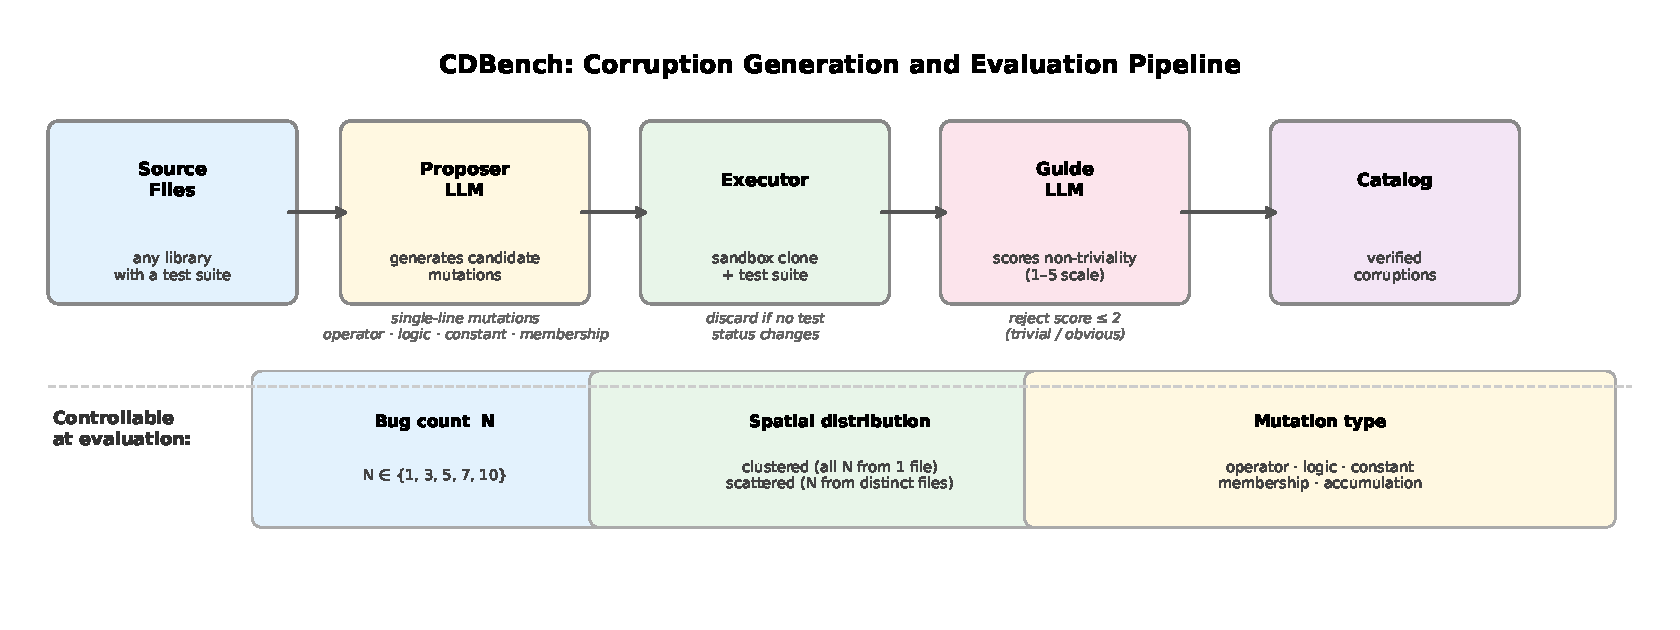
\includegraphics[width=\linewidth]{figs/pipeline.pdf}
\caption{CDBench corruption generation pipeline (top) and the three
  controllable axes at evaluation time (bottom). The Proposer generates
  single-line mutations; the Executor filters for behavioral effect via
  pytest; the Guide rejects trivially-detectable bugs. Bug count $N$,
  spatial distribution, and mutation type can be varied independently.}
\label{fig:pipeline}
\end{figure}

\subsection{Evaluation Protocol}

\paragraph{Group construction.}
For each trial, we sample $N$ corruptions uniformly at random from the catalog.
We stratify by \emph{spatial distribution}: \emph{clustered} groups draw all
$N$ bugs from a single source file---testing whether a model can track multiple
simultaneous faults within a single context---while \emph{scattered} groups draw
from distinct files, requiring cross-file fault localization. Our hypothesis is: co-located bugs share test coverage and API context, while scattered
bugs require the model to reason about disjoint code regions in a single pass.
Results aggregate over both distributions unless noted.

\paragraph{Find-replace output format.}
Prior APR systems use line-level patch formats for single-bug
repair~\cite{xia2024chatrepair,ye2022selfapr}. We adapt this to simultaneous
$N$-bug output: models emit one \texttt{FILE/FIND/FIX} block per bug:

\begin{lstlisting}[basicstyle=\small\ttfamily, frame=single]
FILE: sklearn/metrics/_classification.py
FIND: return np.sum(sample_weight[y_true == y_pred])
FIX:  return np.average(sample_weight[y_true == y_pred])
\end{lstlisting}

Extending this to $N{>}1$ is non-trivial for training: full-file outputs scale
to ${\approx}15\,000$ tokens at $N{=}5$, causing truncated outputs
and zero GRPO gradient from the first training step. The find-replace format
reduces output length to 200--400 tokens at $N{=}5$, eliminating clipping.


\paragraph{Functional scoring.}
Each \texttt{FIND$\to$FIX} substitution is applied to the sandboxed library.
The functional judge runs T\_fail tests for each corruption in the group.
Score $=$ fraction of T\_fail sets fully passing after repair, averaged across
corruptions. This gives per-bug partial credit rather than all-or-nothing
group success.

\paragraph{Held-out evaluation.}
All RL training uses 112 training corruptions. Evaluation uses 27 held-out
corruptions, with group composition drawn from this held-out set. This ensures
no overlap between training and evaluation groups.

\paragraph{Few-shot prompt.}
All models receive a 2-bug few-shot (fs) example demonstrating the \texttt{FILE/FIND/FIX}
format; this abbreviation is used in all table rows (e.g., 7B+fs). This is critical for format compliance at $N{>}1$: without it, 7B
models overwhelmingly emit only one block. We find a scale-dependent sensitivity:
few-shot improves 7B by $+27$\,pp at $N{=}3$ but hurts 3B by $-10$\,pp at
$N{=}1$, suggesting in-context learning capacity for structured format
constraints is itself scale-dependent.

%% ─────────────────────────────────────────────────────────────
\section{Experimental Setup}
\label{sec:setup}

\paragraph{Models.}
We evaluate Qwen2.5-Coder-Instruct~\cite{hui2024qwen25coder} at 3B and 7B
(RL training targets) and Qwen2.5-Coder-32B-Instruct (primary ceiling).
All inference uses vLLM~\cite{kwon2023vllm} with temperature 0.6 and
top\_p$=0.95$ for stochastic runs, greedy for round-0 in iterative experiments.

\paragraph{GRPO training.}
We apply GRPO to Qwen2.5-Coder-7B with:
reward = pytest T\_fail pass rate (0.0--1.0, functional);
$G{=}8$ rollouts per prompt; LoRA~\cite{hu2022lora} rank 16 on all projection matrices;
lr $= 10^{-5}$, cosine decay over 100 steps; training distribution
$N \in \{1, 3, 5\}$ with weights $\{0.5, 0.35, 0.15\}$; 4$\times$H100 GPUs.
Training uses only the 112 training corruptions.

\paragraph{Iterative repair.}
Round 0 uses greedy decoding. Rounds 1--3 use temperature 0.6; the prompt
appends the previous \texttt{FILE/FIND/FIX} output and the names of still-failing
tests. We report \emph{best-of-rounds} (oracle best across all rounds) as the
primary metric, and also per-round incremental rates.

\paragraph{Repair-conditioned GRPO.}
We generate a repair dataset by running the 7B+fs+RL model greedily on 120
training groups (40 per $N \in \{1,3,5\}$). Groups where round-0 score $< 1.0$
become repair examples: the prompt includes the original corrupted code, the
model's previous output, and the still-failing test names. We continue training
from the 7B+fs+RL checkpoint with a 60/40 mix of standard and repair prompts
for 150 steps at lr $= 5{\times}10^{-6}$.

%% ─────────────────────────────────────────────────────────────
\section{Results}
\label{sec:results}

\subsection{Degradation Curves}

\begin{table}[h]
\centering
\caption{Functional debugging accuracy (\%, mean $\pm$ 95\% CI) on
  CDBench held-out set. 32B: 5 trials per $N$; others: 10--20 trials.
  All models use the 2-bug few-shot prompt except 3B/7B base rows.}
\label{tab:baselines}
\begin{tabular}{lcccccc}
\toprule
Model & $N{=}1$ & $N{=}3$ & $N{=}5$ & $N{=}7$ & $N{=}10$ \\
\midrule
3B (no few-shot)          & $40{\pm}32$ & $17{\pm}18$ & $8{\pm}10$  & ---         & ---         \\
3B+fs                     & $30{\pm}30$ & $10{\pm}20$ & $2{\pm}4$   & ---         & ---         \\
7B (no few-shot)          & $60{\pm}32$ & $3{\pm}7$   & $4{\pm}5$   & ---         & ---         \\
7B+fs                     & $70{\pm}30$ & $30{\pm}27$ & $40{\pm}17$ & ---         & ---         \\
\midrule
Qwen2.5-Coder-32B+fs      & $\mathbf{100{\pm}0}$ & $\mathbf{93{\pm}13}$ & $\mathbf{68{\pm}16}$ & $\mathbf{77{\pm}19}$ & $52{\pm}26$ \\
\bottomrule
\end{tabular}
\end{table}

Figure~\ref{fig:degradation} plots the full degradation curves;
Table~\ref{tab:baselines} gives the numeric values with confidence intervals.
All models degrade as $N$ increases. The 32B dense model is the strongest
baseline, degrading most gracefully. Several findings stand out.

\paragraph{Few-shot size sensitivity.}
Few-shot prompting has opposite effects at different scales. For 7B, it
improves $N{=}3$ from 3\% to 30\% (+27\,pp) and $N{=}5$ from 4\% to 40\%
(+36\,pp). For 3B, it hurts $N{=}1$ from 40\% to 30\% and further worsens
multi-fault performance. The 3B model lacks the in-context learning capacity
to generalize the format from the demonstration without degrading its base
behavior. This implies few-shot prompting must be calibrated per model scale.

\begin{figure}[t]
\centering
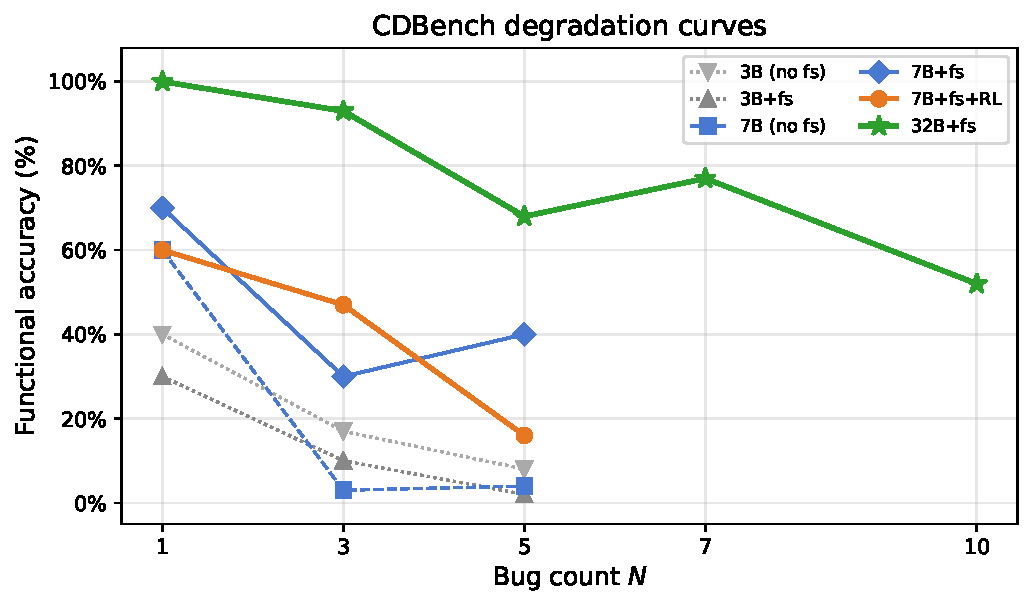
\includegraphics[width=\linewidth]{figs/degradation_curves.pdf}
\caption{Functional debugging accuracy vs.\ bug count $N$. All models degrade
  monotonically; the 32B dense model degrades most gracefully, from 100\%
  at $N{=}1$ to 52\% at $N{=}10$. Smaller models are evaluated at
  $N{\in}\{1,3,5\}$ only; performance had already collapsed to near-zero
  at $N{=}5$, making higher $N$ uninformative for those models.}
\label{fig:degradation}
\end{figure}

\subsection{RL Training Results}

\begin{table}[h]
\centering
\caption{7B+fs+RL vs.\ baselines and ceiling. RL improves $N{=}3$ by 17\,pp
  (30\%$\to$47\%), closing 27\% of the 7B+fs-to-32B gap. All rows: 20 trials.}
\label{tab:rl}
\begin{tabular}{lccc}
\toprule
Model & $N{=}1$ & $N{=}3$ & $N{=}5$ \\
\midrule
7B+fs (baseline)          & 70\% & 30\% & 40\% \\
7B+fs+RL (100 steps)      & 60\% & \textbf{47\%} & 16\% \\
\midrule
32B+fs (ceiling)          & \textbf{100\%} & \textbf{93\%} & \textbf{68\%} \\
Gap closed (7B+fs$\to$32B) & ---  & 27\% & --- \\
\bottomrule
\end{tabular}
\end{table}

At $N{=}3$, the RL-trained model closes 27\% of the gap from the 7B+fs baseline to the 32B ceiling (30\%$\to$47\%, $+17$\,pp; 63\,pp gap reduced to 46\,pp remaining). The $N{=}5$ regression
(40\%$\to$16\%) reflects training distribution dynamics: $N{=}5$ groups have
sparse reward during training (most rollouts score 0), contributing little
gradient, while the model's behavior shifts toward patterns effective at
$N{=}1,3$.

The 3B model with RL (no few-shot, balanced curriculum) improves $N{=}1$ from
40\% to 70\% (+30\,pp) with no regression at $N{=}3$, reaching parity with the
untuned 7B baseline. Few-shot RL training for 3B fails: the few-shot prompt
causes the model to generate 8K+ token outputs (over 80\% of rollouts hit
the token ceiling), indicating the 3B lacks capacity to follow format constraints from
the demonstration under RL generation pressure.

\subsection{Iterative Repair and Repair-Conditioned Training}
\begin{figure}[t]
\centering
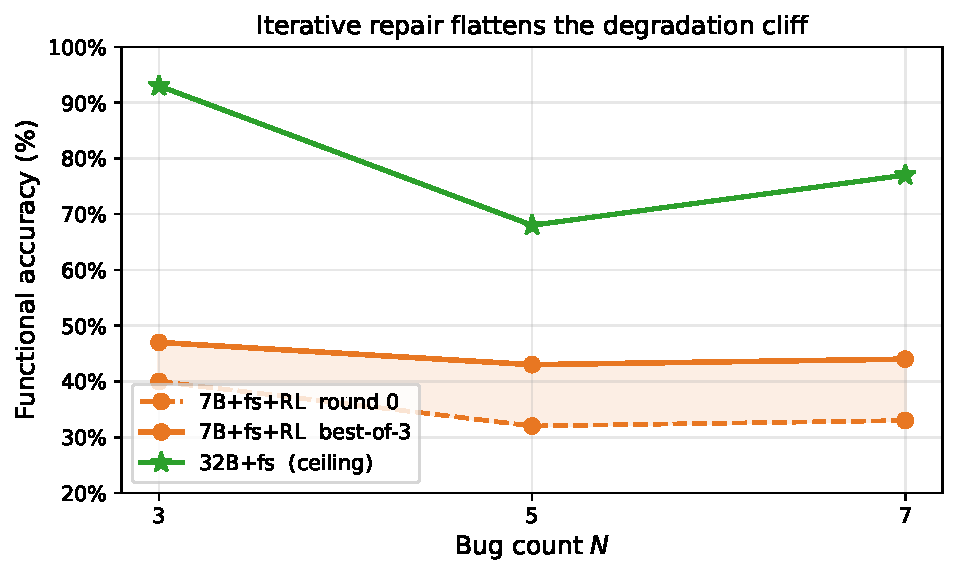
\includegraphics[width=0.75\linewidth]{figs/iterative_repair.pdf}
\caption{Iterative repair (best-of-3 rounds) produces near-flat accuracy
  across $N{=}3$--7, eliminating the degradation cliff visible in the round-0
  curve. The shaded region shows the gain from stochastic re-sampling;
  the 32B ceiling is shown for reference.}
\label{fig:iterative}
\end{figure}

\begin{table}[h]
\centering
\caption{Iterative repair: round-0 vs.\ best-of-3-rounds, and test-name
  ablation (full feedback vs.\ previous attempt only). 20 trials per $N$.}
\label{tab:iterative}
\begin{tabular}{lcccccc}
\toprule
 & \multicolumn{2}{c}{$N{=}3$} & \multicolumn{2}{c}{$N{=}5$} & \multicolumn{2}{c}{$N{=}7$} \\
\cmidrule(lr){2-3}\cmidrule(lr){4-5}\cmidrule(lr){6-7}
 & Round 0 & Best & Round 0 & Best & Round 0 & Best \\
\midrule
7B+fs+RL (full feedback)  & 40\% & 47\%  & 32\% & 43\%  & 33\% & 44\%  \\
7B+fs+RL (prev only)      & 40\% & 43\%  & 32\% & 43\%  & 33\% & 41\%  \\
32B+fs                    & 93\% & 93\%  & 68\% & 68\%  & 77\% & 77\%  \\
\bottomrule
\end{tabular}
\end{table}

Iterative repair adds 7--11\,pp at $N{=}3$--7, producing near-flat accuracy
(43--47\%) across that range. Repair success saturates after round 1: hard
groups remain hard across all subsequent attempts. Test names contribute only
$\sim$6\,pp at $N{=}3$ and nothing at $N{=}5$; the dominant gain is stochastic
exploration at temperature 0.6. Best-of-rounds is therefore equivalent to
best-of-$k$ sampling---the gain could be realized via parallel sampling without
a sequential feedback loop.

\begin{table}[h]
\centering
\caption{Repair-conditioned training vs.\ 7B+fs+RL baseline. Round-0 and
  best-of-3-rounds accuracy. 20 trials per $N$.}
\label{tab:repair}
\begin{tabular}{lcccccc}
\toprule
 & \multicolumn{2}{c}{$N{=}1$} & \multicolumn{2}{c}{$N{=}3$} & \multicolumn{2}{c}{$N{=}5$} \\
\cmidrule(lr){2-3}\cmidrule(lr){4-5}\cmidrule(lr){6-7}
 & Round 0 & Best & Round 0 & Best & Round 0 & Best \\
\midrule
7B+fs+RL (baseline)   & 60\% & 60\% & 40\% & 47\% & 32\% & 43\% \\
7B+fs+RL+repair       & 50\% & 50\% & \textbf{58\%} & \textbf{60\%} & 33\% & \textbf{46\%} \\
$\Delta$ vs.\ baseline & $-10$\,pp & 0 & $+18$\,pp & $+13$\,pp & $+1$\,pp & $+3$\,pp \\
\bottomrule
\end{tabular}
\end{table}

\begin{figure}[t]
\centering
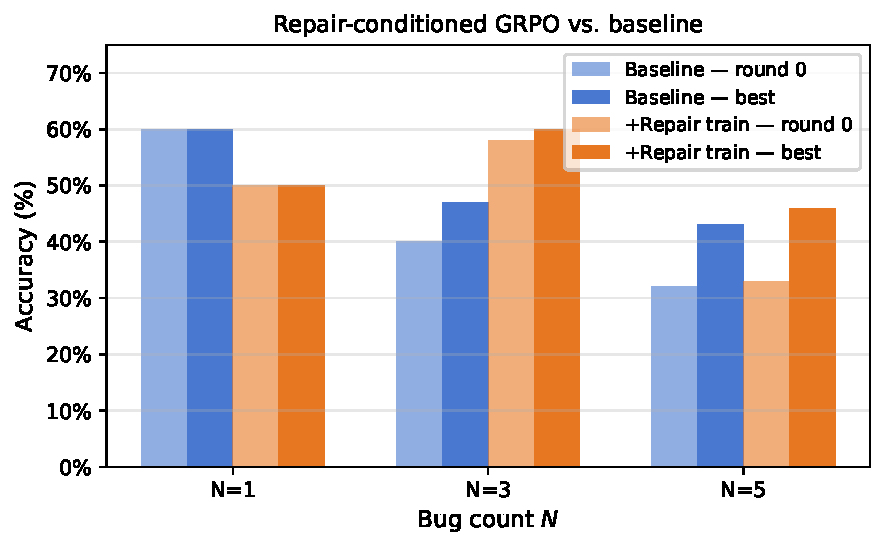
\includegraphics[width=0.75\linewidth]{figs/repair_training.pdf}
\caption{Repair-conditioned GRPO (7B+fs+RL+repair) vs.\ baseline (7B+fs+RL).
  $N{=}3$ gains $+18$\,pp single-shot from tractable repair examples;
  $N{=}5$ gains only in iterative rounds via format transfer;
  $N{=}1$ regresses due to distribution shift toward hard failures.}
\label{fig:repair}
\end{figure}

Repair-conditioned training produces asymmetric gains: $+18$\,pp at $N{=}3$
(single-shot, before any repair context), $+1$\,pp at $N{=}5$, and $-10$\,pp
at $N{=}1$. The asymmetry follows from GRPO gradient quality. The repair
dataset consists of past failures, and the difficulty of those failures varies
sharply: $N{=}1$ examples are complete failures (0 remaining bugs fixed),
$N{=}3$ examples average 2.25 remaining bugs, and $N{=}5$ examples average
3.6. GRPO requires nonzero reward variance across its $G{=}8$ rollouts to
produce a gradient; when the model almost never succeeds on a repair example,
all rollouts return the same score and no learning occurs. $N{=}3$ repair
examples sit in the tractable regime---the model occasionally completes them,
gradient flows, and learned priors transfer to single-shot $N{=}3$ performance.
$N{=}5$ repair examples are too hard; the $+3$\,pp iterative gain there comes
from format transfer learned on $N{=}3$ examples, not from $N{=}5$-specific
gradient. This has a design implication: repair examples must be sampled from the
difficulty regime where the model can occasionally succeed.
%% ─────────────────────────────────────────────────────────────
\subsection{Cross-Library Transfer}
\label{sec:transfer}

To test whether RL-trained debugging behavior generalizes across domains, we
evaluate the sklearn-trained 7B+fs+RL model on 30 SciPy corruptions (from
\texttt{scipy.stats} and \texttt{scipy.optimize}) without any SciPy-specific
RL training. We compare against a 7B+fs baseline and a 32B+fs ceiling, each
evaluated on the same pool.

\begin{table}[h]
\centering
\caption{Zero-shot transfer to SciPy. The 7B+RL model was trained exclusively
  on scikit-learn; no SciPy-specific training was performed. Metric: mean fraction
  of bugs fixed per trial (same partial-credit metric as Table~\ref{tab:baselines}).
  7B models: 40 trials per $N$; 32B: 20 trials.}
\label{tab:scipy}
\begin{tabular}{lccc}
\toprule
Model & $N{=}1$ & $N{=}3$ & $N{=}5$ \\
\midrule
7B+fs (baseline)          & 35\% & 62\% & 56\% \\
7B+fs+RL (sklearn-trained) & \textbf{43\%} & 52\% & 47\% \\
\midrule
32B+fs (ceiling)          & \textbf{75\%} & \textbf{68\%} & \textbf{63\%} \\
\bottomrule
\end{tabular}
\end{table}

RL training on scikit-learn partially transfers to SciPy: $N{=}1$ improves
from 35\% to 43\% ($+7.5$\,pp), indicating that the basic single-bug
debugging prior generalizes across library domains. However, the $N{=}3$
benefit does not transfer---the RL model regresses to 52\% (from the 62\%
baseline, $-10$\,pp), widening rather than closing the gap to the 32B ceiling
at that fault count. This suggests the RL model learned scikit-learn-specific
bug patterns during training rather than a general multi-fault strategy.
Inspection of the training corpus suggests a mechanism: 54\% of the 112
training corruptions are simple operator or constant perturbations
(\texttt{comparison\_flip}, \texttt{arith\_operator}, \texttt{logic\_operator},
\texttt{constant\_change}), and RL rewards this fix vocabulary heavily.
SciPy bugs involve similar surface-level patterns but with different
domain semantics (library-specific variable names, array conventions, numerical
thresholds). The RL model applies its learned sklearn fix vocabulary in the
wrong contexts: outputs on SciPy show confident comparison flips and operator
changes even when the fix requires different domain knowledge, which degrades
multi-fault performance where compound errors amplify each mismatch.

The 32B ceiling itself drops substantially from scikit-learn ($N{=}1$: 100\%
$\to$ 75\%) to SciPy, confirming that SciPy corruptions present distinct
challenges even for strong baselines. Three questions follow for future work.
First, \emph{near-vs-far domain transfer}: scikit-learn and SciPy share NumPy
array conventions and similar test structures; a near-far spectrum could test
whether transfer degrades continuously with domain distance (scikit-learn
$\to$ SciPy $\to$ Django $\to$ embedded C). Second, \emph{multi-domain training}:
mixing scikit-learn and SciPy corruptions during RL may improve transfer
without sacrificing in-domain performance. Third, \emph{domain-adaptive reward}:
a library-agnostic reward signal (e.g., test coverage delta rather than
library-specific pytest pass rate) may produce more transferable policies.

\paragraph{Limitations and open questions.}
The held-out evaluation set is 27 corruptions, which limits statistical power;
the wide confidence intervals in Table~\ref{tab:baselines} reflect this, and
results should be interpreted as directional rather than definitive. Scaling the
benchmark---more corruptions, more libraries---is the clearest path to
higher-confidence claims, and is the motivation for releasing CDBench as
extensible infrastructure. The iterative repair oracle (best-of-rounds) requires
knowing which round was best at evaluation time; a deployed system would need a
stopping criterion or a verifier. Finally, all RL experiments use a
single model family (Qwen2.5-Coder) and a single domain (scikit-learn);
generalization of the training recipe to other architectures and domains is
assumed but not demonstrated.

%% ─────────────────────────────────────────────────────────────
\section{Conclusion}
\label{sec:conclusion}

CDBench makes bug count a tunable proxy for sequential reasoning depth. Key
findings: (1) all models degrade monotonically with $N$---even the 32B ceiling
drops from 100\% at $N{=}1$ to 52\% at $N{=}10$, suggesting sequential task
complexity is the binding constraint; (2) GRPO with functional reward improves
$N{=}3$ by 17\,pp, closing 27\% of the 7B+fs-to-32B gap; (3) iterative repair
is equivalent to best-of-$k$ sampling, eliminating the degradation cliff at
$N{=}3$--7; (4) repair-conditioned training requires tractable repair examples
to produce gradient---this criterion explains the asymmetric gains across $N$;
(5) zero-shot transfer to SciPy shows the $N{=}1$ gain generalizes but the
$N{=}3$ gain does not, pointing to multi-domain training as a necessary next step.

Format design, inference-time compute, and training signal tractability are more
predictive of multi-fault debugging performance than raw model scale. CDBench is
released as extensible infrastructure: the SGS pipeline generates corruptions
for any library with a test suite.



\bibliographystyle{unsrtnat}
\bibliography{references}

\end{document}
